\documentclass{article}
\usepackage[utf8]{inputenc}
\usepackage{amsmath}
\usepackage{amssymb}
\usepackage{float}
\usepackage{graphicx}
\usepackage{anysize}
\usepackage{amsthm}
\usepackage{dsfont}
\usepackage{marvosym}
\usepackage{enumitem}
\usepackage{wrapfig}%paquete para manejar gráficas al lado de texto

% Controla los márgenes {izquierda}{derecha}{arriba}{abajo}. 
\marginsize{2.7cm}{2.1cm}{2.8cm}{3.5cm}

\renewcommand{\figurename}{Figura}
\renewcommand\refname{}
\renewcommand{\thesection}{\arabic{section}.} %instrucción para modificar la numeración de las secciones
\renewcommand{\thesubsection}{\arabic{section}.\arabic{subsection}.}
\renewcommand{\theequation}{\arabic{section}.\arabic{equation}} 

\allowdisplaybreaks[4] % Permite separar una ecuación en dos páginas

\title{\textsc{\Large{Métodos computacionales - Tarea 1}}}
\author{\textsc{\Large{Diego Gomez}}\hspace{10pt}(201318237)}
\date{}

\begin{document}

    \maketitle

    \begin{figure}
        \centering
        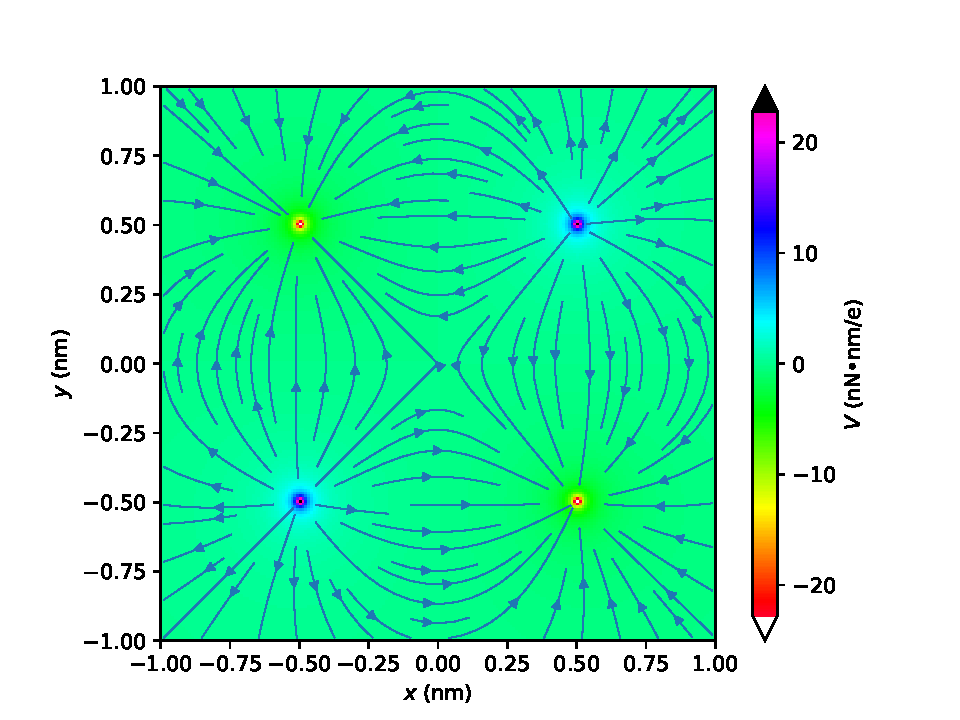
\includegraphics[width=0.7\textwidth]{cargas.pdf}
        \caption{Potencial y campo generado por 4 cargas.}
        \label{fig:cargas}
    \end{figure}
    
    \begin{figure}
        \centering
        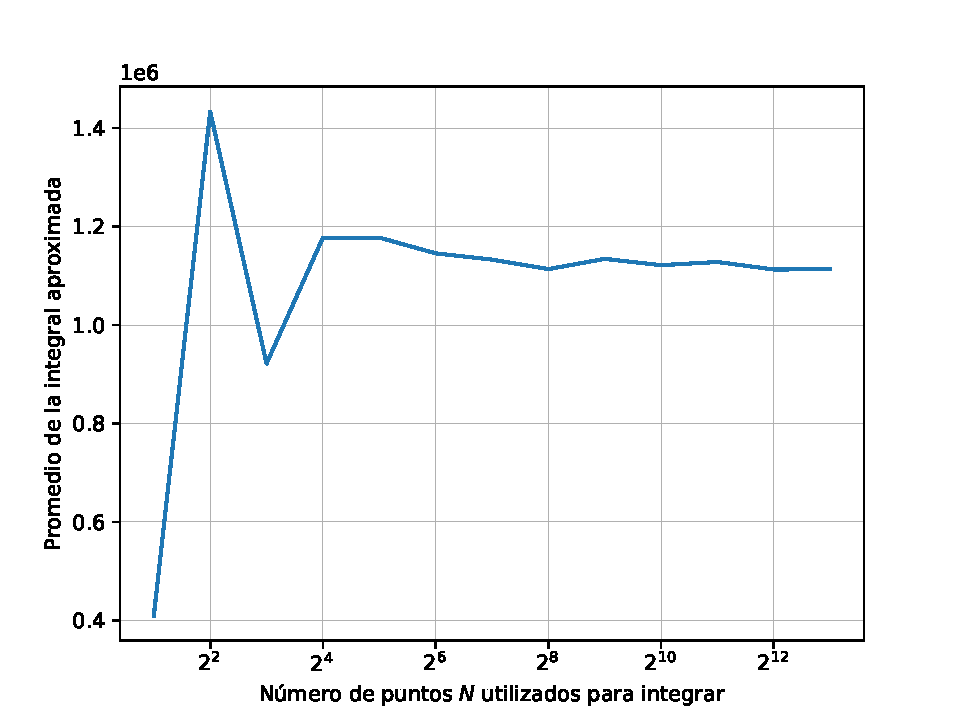
\includegraphics[width=0.7\textwidth]{num_integral.pdf}
        \caption{Aproximación de la integral.}
        \label{fig:num_integral}
    \end{figure}

    \begin{figure}
        \centering
        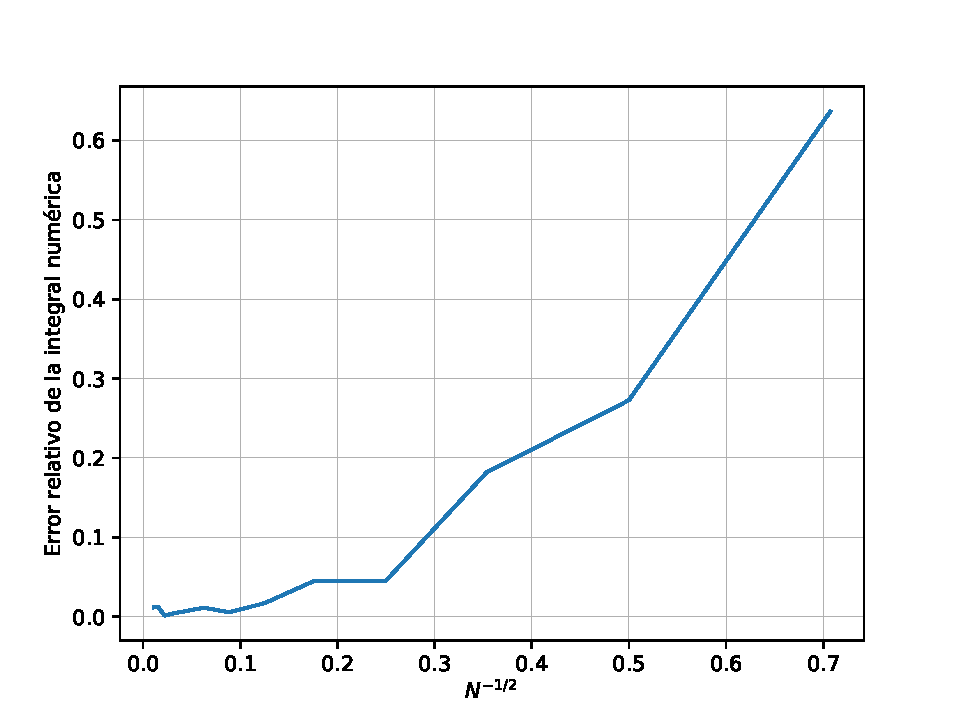
\includegraphics[width=0.7\textwidth]{err_integral.pdf}
        \caption{Error de la integral.}
        \label{fig:err_integral}
    \end{figure}    

\end{document}
